\documentclass[11pt,landscape]{article}
\usepackage{multicol}
\usepackage{calc}
\usepackage{ifthen}
\usepackage[landscape]{geometry}
\usepackage{hyperref}
\usepackage{lipsum}  

\ifthenelse{\lengthtest { \paperwidth = 11in}}
	{ \geometry{top=.5in,left=.5in,right=.5in,bottom=.5in} }
	{\ifthenelse{ \lengthtest{ \paperwidth = 297mm}}
		{\geometry{top=1cm,left=1cm,right=1cm,bottom=1cm} }
		{\geometry{top=1cm,left=1cm,right=1cm,bottom=1cm} }
	}

% Turn off header and footer
\pagestyle{empty}
 \usepackage{amsmath}

% Redefine section commands to use less space
\makeatletter
\renewcommand{\section}{\@startsection{section}{1}{0mm}%
                                {-1ex plus -.5ex minus -.2ex}%
                                {0.5ex plus .2ex}%x
                                {\normalfont\large\bfseries}}
\renewcommand{\subsection}{\@startsection{subsection}{2}{0mm}%
                                {-1explus -.5ex minus -.2ex}%
                                {0.5ex plus .2ex}%
                                {\normalfont\normalsize\bfseries}}
\renewcommand{\subsubsection}{\@startsection{subsubsection}{3}{0mm}%
                                {-1ex plus -.5ex minus -.2ex}%
                                {1ex plus .2ex}%
                                {\normalfont\small\bfseries}}
\makeatother

% Define BibTeX command
\def\BibTeX{{\rm B\kern-.05em{\sc i\kern-.025em b}\kern-.08em
    T\kern-.1667em\lower.7ex\hbox{E}\kern-.125emX}}

% Don't print section numbers
\setcounter{secnumdepth}{0}
\usepackage{circuitikz}


\setlength{\parindent}{0pt}
\setlength{\parskip}{0pt plus 0.5ex}
\usepackage{karnaugh-map}


% -----------------------------------------------------------------------

\begin{document}

\raggedright
\footnotesize
\begin{multicols*}{3}


% multicol parameters
% These lengths are set only within the two main columns
%\setlength{\columnseprule}{0.25pt}
\setlength{\premulticols}{1pt}
\setlength{\postmulticols}{1pt}
\setlength{\multicolsep}{1pt}
\setlength{\columnsep}{2pt}

\begin{center}
     \Large{\textbf{ECE253 Midterm Cheatsheet}} \\
\end{center}



\section{Boolean Algebra}
\textbf{De Morgan's Theorem} tells us
\begin{equation}
    \overline{x\cdot y}=\overline{x}+\overline{y}, \quad\quad\quad \overline{x+y}=\overline{x}\cdot\overline{y}
\end{equation}
Inverting the inputs to an \verb!or! gate is the same as inverting the outputs to an \verb!and! gate, and the other way around. We also have: 
\begin{itemize}
    \item $(x+y)(y+z)(\overline{x}+z)=(x+y)(\overline{x}+z)$
    \item $x+yz=(x+y)(x+z)$
    \item $x+xy=x$ (Absorption)
    \item $xy+x\overline{y}=x$ (Combining)
    \item $(x+y)(x+\overline{y})=x$
    \item $ x+\overline{x}y=x+y$
    \item $x(\overline{x}+y)=xy$
    \item $xy+yz+z\overline{x}=xy+z\overline{x}$ (Consensus)
\end{itemize}

\subsection{Gates}
\begin{center}
    \begin{tabular}{c|c||c|c||c|c}
        \verb!AND! & \begin{circuitikz}[scale=0.7, transform shape] 
            \draw(0,0) node[and port] {};
        \end{circuitikz} & 

        \verb!OR! & \begin{circuitikz}[scale=0.7, transform shape] 
            \draw(0,0) node[or port] {};
        \end{circuitikz} &
        \verb!NOT! & \begin{circuitikz}[scale=0.7, transform shape] 
            \draw(0,0) node[not port] {};
        \end{circuitikz} \\ \hline
        \verb!NOR! & \begin{circuitikz}[scale=0.7, transform shape] 
            \draw(0,0) node[nor port] {};
        \end{circuitikz} &
        \verb!NAND! & \begin{circuitikz}[scale=0.7, transform shape] 
            \draw(0,0) node[nand port] {};
        \end{circuitikz} &
        \verb!XOR! & \begin{circuitikz}[scale=0.7, transform shape] 
            \draw(0,0) node[xor port] {};
        \end{circuitikz}
    \end{tabular}
\end{center}
\subsection{SOPs and POSs}
We can create boolean algebra expressions for truth tables.
\vspace{2mm}

\textbf{Minterm:} Corresponds to each row of truth table, i.e. $m_3=\overline{x_2}x_1x_0$ such that when $3=0b011$ is substituted in, $m_3=1$ and $m_3=0$ otherwise.  

\textbf{Maxterm:} They give $M_i=0$ if and only if the input is $i$. For example, $M_3=x_2+\overline{x_1}+\overline{x_0}.$

\textbf{SOP and POS:} Truth tables can be represented as a sum of minterms, or product of maxterms.
\begin{itemize}
    \item Use minterms when you have to use \verb!NAND! gates and maxterms when you have to use \verb!NOR! gates.
    \item When converting expressions to its dual, it's often helpful to negate expressions twice, or draw out the logic circuit.
\end{itemize}
\subsection{Cost}
The cost of a logic circuit is given by
\begin{equation}
    \text{cost} = \text{gates} + \text{inputs}
\end{equation}
If an inversion (\verb!NOT!) is performed on the primary inputs, then it is not included. If it is needed inside the circuit, then the \verb!NOT! gate is included in the cost.
\subsection{Karnaugh Map}
Method of finding a minimum cost expression: We can map out truth table on a grid for easier pattern recognition. Example of a four variable map is shown below:
\begin{center}
    \begin{karnaugh-map}[4][4][1][$x_2x_1$][$x_4x_3$]
        \minterms{0,1,3,4,5,7,11,14,15,10}
        \maxterms{2,6,8,9,10,12,13}
        % \indeterminants{2,5}
        \implicant{0}{5}
        \implicant{3}{11}
        \implicant{15}{10}
        % \implicant{4}{5}
    \end{karnaugh-map}
\end{center}
\vspace{-8mm}
and the representation is $\overline{x_2}\cdot\overline{x_4}+x_2 \cdot x_1+\overline{x_4} \cdot x_2$ when using \textit{minterms}. To use \textit{maxterms}, we take the intersection of sets that don't include blocks of $0$s. For example, $(\overline{x_2}\cdot \overline{x_1})(\overline{x_2}+x_1+x_4).$ Some \textit{rules}: 
\begin{itemize}
    \item Side lengths should be powers of $2$ and be as large as possible.
    \item Use \textbf{graycoding}: adjacent rows/columns should share one bit.
\end{itemize}
\subsubsection{Minimization Procedure}
\begin{enumerate}
    \item Generate all prime implicants for given function $f$
    \item Find the set of essential prime implicants
    \item Determine the nonessential prime implicants that should be added.
\end{enumerate}
\subsection{Common Logic Gates}
\begin{itemize}
    \item \textbf{Mux 2$\rightarrow$1:} $\verb#mux2to1#(s,x_0,x_1) = \overline{s}x_0+sx_1$
    \item \textbf{Not:} \verb#not(x)=nand(x,x)=nor(x,x)#
    \item \verb!XOR! acts as modular arithmetic.
    \item Multiplexers are functionally complete. $\verb!AND!=mux(x,y,1)$, $\verb!OR!=mux(x,0,y).$
\end{itemize}
\subsection{RS Latch}
Sequential circuits depend on sequence of inputs. A \textbf{SR Latch} are cross-coupled \verb!NOR! gates.
\vspace{2mm}
% \begin{center}
    {
    \begin{multicols}{2}
        \begin{center}
            \begin{circuitikz} \draw
                (0,2) node[nor port] (NOR1) {}
                (1,2) node[anchor=east] {Q}
                (1,0) node[anchor=east] {$\overline{Q}$}
                (0,0) node[nor port] (NOR2) {}
                (NOR1.in 1) node[anchor=east] {R}
                (NOR2.in 2) node[anchor=east] {S}
                (NOR1.out) -- ++(0,-0.5) -- ($(NOR2.in 1) +(0,0.5)$) -- (NOR2.in 1)
                (NOR2.out) -- ++(0,+0.5) -- ($(NOR1.in 2) +(0,-0.5)$)--(NOR1.in 2)
                ;\end{circuitikz}
        \end{center}


        \begin{center}
            \begin{tabular}{c|c|c|c}
                S & R & Q & $\overline{Q}$ \\ \hline
                0 & 0 & 0/1 & 1/0 \\
                0 & 1 & 0 & 1 \\ 
                1 & 0 & 1 & 0 \\ 
                1 & 1 & 0 & 0
           \end{tabular}
        \end{center}
        \vspace{-2mm}
        \scriptsize When $S=R=0$, it stores the last $Q$ value. In practice, we should not have $S=R=1$.
    \end{multicols}
}
\subsection{Gated D Latch and Clock Signal}
{
    \begin{multicols}{2}
        \begin{center}
            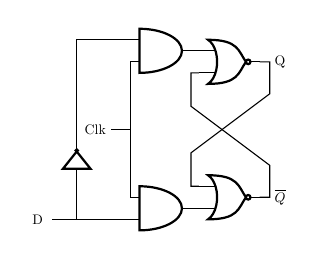
\begin{tikzpicture}[scale=0.5, transform shape]
 
                % Draw and gates
                \node[and port] (and1) at (0,2) {};
                \node[and port] (and2) at (0,-2) {};
                 
                % Draw nor gates
                \draw (and1.out) -- ++(0.2,0) node
                [
                    nor port,
                    anchor=in 1
                ] (nor1) {};
                 
                \draw (and2.out) -- ++(0.2,0) node
                [
                    nor port,
                    anchor=in 2
                ] (nor2) {};
                 
                \draw (nor1.in 2) -| ++ (-0.2,-0.85) -- ++(2,-1.5) coordinate(a) |- (nor2.out);
                \draw (nor2.in 1) -| ++ (-0.2,0.85) -- ++(2,1.5) |- (nor1.out);
                 
                % Clock
                \draw (and1.in 2) -- (and2.in 1)node[midway](clk){};
                \draw (clk.center) -- ++(-0.5,0) node[left]{Clk};
                 
                % Output labels
                \draw (nor1.out -| a) node[right]{Q};
                \draw (nor2.out -| a) node[right]{$\overline{Q}$};
                 
                \draw (and2.in 2) -- ++(-2,0) coordinate(a2) node[left=0.1cm]{D};
                 
                % Not port
                \node
                [
                    not port,
                    rotate=90,
                    scale=0.5,
                ](not) at (-2.75,-0.75){};
                 
                \draw (not.in) |- (a2) (not.out) |- (and1.in 1)  ;
                 
                \end{tikzpicture}
        \end{center}


        \begin{center}
            \begin{tabular}{c|c}
                Clk & $Q(t+1)$ \\ \hline
                0 & Q(t) \\
                1 & D
           \end{tabular}
        \end{center}
        \vspace{-3mm}
    \end{multicols}
}

% \end{center}
\subsection{D Flip Flops}
Consists of two gated D latches, connected in series and both connected to the same clock. However, clock input for the first D latch is inverted. When the clock rises up, $Q$ stores value of $D$.
\subsection{T Flip Flops}
\begin{multicols}{2}
    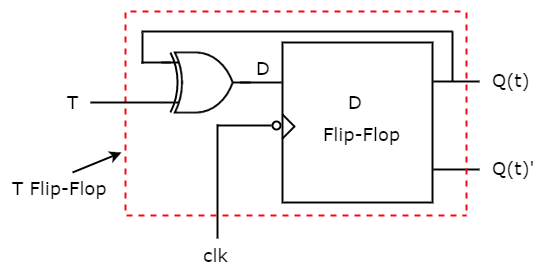
\includegraphics[width=1.1\linewidth]{figures/T.png}
    \begin{center}
        \begin{tabular}{c|c|c}
        clk & $Q(t+1)$ \\ \hline
        $\uparrow$ & \verb!T^Q(t)! 
   \end{tabular}
    \end{center}
\end{multicols}
\subsection{Verilog}
\subsubsection{Logic Operators}
\begin{center}
    \begin{tabular}{c|c||c|c}
        \verb!bitwise AND! & \verb!&! &
        \verb!bitwise OR! & \verb!|! \\ \hline
        \verb!bitwise NAND! & \verb!~&! &
        \verb!bitwise NOR! & \verb!~!!  \\ \hline
        \verb!bitwise XOR! & \verb!^! &
        \verb!bitwise XNOR! & \verb!~^! \\ \hline
        \verb!logical negation! & \verb!!! &
        \verb!bitwise negation! & \verb!~! \\ \hline 
        \verb!concatenation! & \verb!{}! &
        \verb!replication! & \verb!{{}}! 
    \end{tabular}
\end{center}
\begin{itemize}
    \item \verb!reduction! operators are put at the start and output a scalar.
    \item \verb!bitwise! operators 
    \item \verb!blocking assignment =!: executed in the order they are specified.
    \item\verb!Nonblock assignments <=! executed in parallel.
\end{itemize}
\newpage 
\subsubsection{Case Statements}
\begin{verbatim}
module mux(MuxSelect, Input, Out);
    input [4:0] Input; input [2:0] MuxSelect;
    output Out;
    reg Out; // declare output for always block
    always @(*) // declare always block
    	begin
    	case (MuxSelect[2:0]) // start case statement
    	3'b000: Out = Input[0]; // case 0
    	// ...
    	3'b100: Out = Input[4]; // case 4
    	default: Out = 1'bx; // default case
    	endcase end endmodule
\end{verbatim}
\subsubsection{Half Adder}
\begin{verbatim}
module HA(x, y, s, c);
    input x, y; output s, c;
    assign s = x^y;
    assign c = x&y;
endmodule
\end{verbatim}
\subsubsection{Full Adder}
\begin{verbatim}
module FA(a, b, c_in, s_out, c_out);
    input a, b, c_in; output s_out, c_out;
    wire w1, w2, w3;
    HA u0(.x(a), .y(b), .s(w1), .c(w2));
    HA u1(.x(c_in), .y(w1), .s(s_out), .c(w3));
    assign c_out = w2|w3;
endmodule
\end{verbatim}
\subsection{D Flip Flop}
\begin{verbatim}
module D-ff(D, clk, Q);
    input D, clk;
    output reg Q;   
    always@(posedge clk) Q <= D; // use <= operator
endmodule
\end{verbatim}
\subsection{Flip Flop (stores on both edges)}
\begin{verbatim}
module DDR (input c, input D, output Q) ;
    reg p, n;
    always @ (posedge c) p <= D;
    always @ (negedge c) n <= D;
    assign Q <= c ? p : n;
endmodule
\end{verbatim}
\subsection{Registers}
\begin{verbatim}
module reg8(D, clk, Q);
    input clock;
    input [7:0] D;
    output reg[7:0] Q;
    always@(posedge clock)
        Q <= D;
    endmodule
\end{verbatim}
\subsection{ModelSim Do Files}
\begin{verbatim}
# set working dir, where compiled verilog goes
vlib work
# compile all verilog modules in mux.v to working
# dir could also have multiple verilog files
vlog mux.v
#load simulation using mux as the
# top level simulation module
vsim mux
#log signals and add signals to waveform window
log {/*}
# add wave {/*} would add all items in
# top level simulation module
add wave {/*}
# set input values using the force command
# signal names need to be in {} brackets
force {SW[0]} 0
force {SW[1]} 0
run 10ns
\end{verbatim}
\textbf{ModelSim and Other Lab Things}
\begin{itemize}
    \item FGPA: Field Programmable Gate Array
    \item To repeat signals, use this syntax: 
    \begin{verbatim}
force {MuxSelect[2]} 0 0ns, 1 {4ns} -r 8ns
    \end{verbatim}
    \vspace{-4mm}
    which starts at $0$ at 0ns, $1$ at 4ns, and repeats every $8$ ns.
    \item On the \verb!DE1-SoC! board, hex thing is red if $0$ and white if $1$.
\end{itemize}
\subsection{Frequency Dividers}
\begin{itemize}
    \item To half the frequency, connect $\overline{Q}$ to $D$ on the same gated D latch.
    \item To quarter the frequency, connect $\overline{Q}$ to the clock of the next gated D latch (which is set up the same as the half frequency case).
    \item To reduce frequency by $2k$, connect $k$ D latches connected in series ($D$ to $Q$) and to the same clock. First $D$ is connected to last $\bar{Q}$. The last $Q$ will have a reduced frequency of $2k$.
\end{itemize}
\subsection{Resets}
\begin{itemize}
    \item Active High/Low: Resets when Signal is 1/0
    \item Synchronous High/Low: Resets during positive/negative edge
\end{itemize}
\section{Finite State Machines}
\subsection{Steps}
\begin{multicols}{2}
    \begin{enumerate}
        \item State Diagram
        \item State Table
        \item State Assignment
        \item State-Assigned Table
        \item Synthesize Circuit
        \item Celebrate!
    \end{enumerate}
\end{multicols}
\subsection{Step 1: State Diagram Example}
\begin{center}
    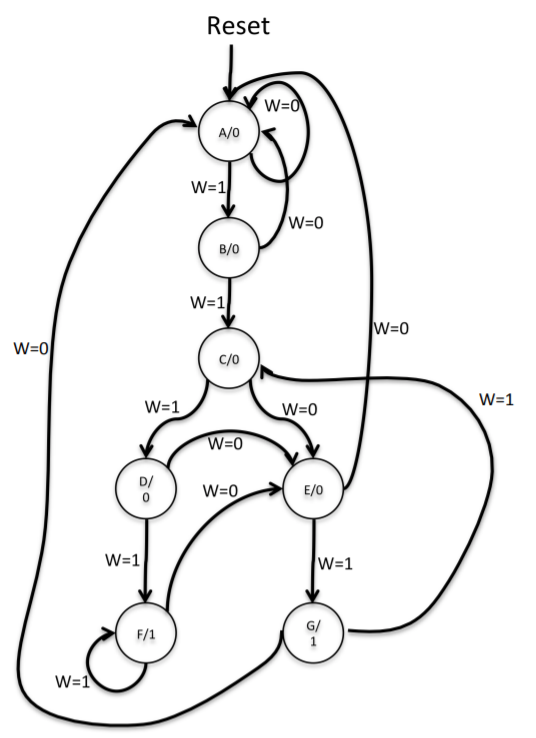
\includegraphics[width=0.6\linewidth]{figures/fsm.png}
\end{center}
\subsection{Step 2: State Table Example}
\begin{center}
    \begin{tabular}{c|cc|c}
        Present State & \multicolumn{2}{c|}{Next State} & Output ($z$) \\ 
        A & A & B& 0 \\ 
        B & A & C & 0 \\ 
        $\vdots$ & $\vdots$ & $\vdots$ & $\vdots$ \\
        G & A & C & 1
    \end{tabular}
\end{center}
\subsection{Step 3: State Assignment Example}
\begin{itemize}
    \item Using \textbf{one-hot encoding:} Choose number of flip flops: $7$ (since 7 states)
    \item Choose state codes:
    \begin{itemize}
        \item A = 0000001, B=0000010, $\dots$, G=1000000
    \end{itemize}
\end{itemize}
Alternatively use 3 flip flops to represent state codes as 000, 001, 010, etc.

\newpage 

\subsection{Step 4: State-Assigned Table Example}
By convention, use $y$ for input and $Y$ for output.
\begin{tabular}{c|cc|c}
    $y_3y_2y_1$ & $Y_3Y_2Y_1$ $(W=0)$ & $Y_3Y_2Y_1$ $(W=1)$ & z \\ 
    000 & 000 & 001 & 0 \\ 
    001 & 000 & 010 & 0 \\
    $\vdots$ & $\vdots$ & $\vdots$ & $\vdots$ \\
    110 & 000 & 010 & 1
\end{tabular}
\subsection{Step 5: Synthesize Example}
We first write boolean algebra expressions for the outputs $Y_n=f_n(y_1,y_2,y_3,W$) and $z=g(y_1,y_2,y_3)$. For each flip flop $i$, the input is $Y_i$ and the output is $y_i$. The output then branches off into two paths:
\begin{itemize}
    \item The first path goes into the function $g(y_1,y_2,y_3)$ and leads to output $z$
    \item The second path goes into the function $f_nm(y_1,y_2,y_3,W)$ and \textbf{loops back} to $Y_n.$
\end{itemize}
The D flip flops are connected to same clock and reset signal.
\subsection{Execution in Verilog}
\begin{verbatim}
module FSM(input Clock, input Resetn, input w,
           output z, output [3:0] CurState);

reg [3:0] y_Q, Y_D;
localparam A=4'b0000, B=4'b0001, ... , G=4'b0110

always@(*) // State Table
begin: state_table
    case: (Y_Q)
        A: begin
                if (!w) Y_D = A; else Y_D = B;
           end
        // ...
        G: begin
                if (!w) Y_D = A; else Y_D = C;
        default: Y_D = A;
    endcase
end 

always @(posedge Clock) // State Registers
begin: state_FFs
    if(Resetn == 1'b0) y_Q <= A;
    else y_Q <= Y_D;
end

// Output Logic
assign z = ((y_Q == F) | (y_Q == G));
assign CurState = y_Q;
endmodule
\end{verbatim}
\section{ARM Assembly}
\subsection{Registers}
\begin{itemize}
    \item R0-R3: Scratch Registers: will be overwritten by subroutines.
    \item R4-R12: Preserved Registers: stack before using, restore before returning
    \item R13 (SP): Stack Pointer: points to top of stack
    \item R14 (LR): Link Register (Points to return address when BL is executed
    \item R15 (PC): Program Counter: Holds address of next instruction to execute
\end{itemize}
\subsection{Instructions}
Let \verb!r0=1!, \verb!r1=2!, \verb!r2=#0b1010!.
\vspace{-0mm}
\begin{center}
    \begin{tabular}{c|c|c}
    Instruction & Example & Result \\ 
    \verb!MOV! & \verb!mov r3, #3    ! & \verb!r3 = 3     !\\ 
    \verb!ADD! & \verb!add r3, r0, r0! & \verb!r3 = 1 + 1 !\\
    \verb!SUB! & \verb!sub r3, r0, r0! & \verb!r3 = 1 - 1 !\\
    \verb!MUL! & \verb!mul r3, r0, r0! & \verb!r3 = 1 * 1 !\\
    \verb!LSL! & \verb!lsl r3, r2, #1! & \verb!r3 = #0b0100! \\ 
    \verb!LSR! & \verb!lsr r3, r2, #1! & \verb!r3 = #0b0101! \\
    \verb!ASR! & \verb!asr r3, r2, #1! & \verb!r3 = #0b1101! \\
    \verb!AND! & \verb!and r3, r1, r0! & \verb!r3 = (1 and 2) = 0! \\
    \end{tabular}
\end{center}
\subsection{Memory Stuff}
\begin{itemize}
    \item \verb!BL:Branch Link!: Goes to a branch but updates \verb!LR!
    \item Stacks: \verb!PUSH {R0, R1}! pushes \verb!R0,R1! to a stack where \verb!R0! is at the top. Last in First Out.
    \item Each instruction is a place in memory, with addresses going up by 4 bytes.
    \item Addresses of inputs are stored in the memory immediately after the instructions.
\end{itemize}
\subsection{Load and Store}
\begin{itemize}
    \item \verb!LDR Ra, [Rb], #offset!: value at [address] found in \verb!Rb! is loaded into register \verb!Ra!. Then the [address] is incremented by \verb!offset!.
    \item \verb!STR Ra, [Rb], #offset!: value found in register \verb!Ra! is stored to [address] found in \verb!Rb!. Then the [address] is incremented by \verb!offset!.
    \item \verb!LDR Ra, =LIST! Makes \verb!Ra! contain the address to the first element of the input variable.
\end{itemize}
\textbf{Fancy Stuff:}
\begin{itemize}
    \item \verb!LDR Ra, [Rb, #offset]! is pre-indexed (doesn't change Rb)
    \item \verb!LDRB! - load byte (8 bits, which is 2 hex letters)
    \item \verb!LDRSB! - signed load byte (LDRB but gives sign extension to result to make it 4 bytes while retaining the sign)  
    \item \verb!LDRH! - load halfword (for \verb![R3, #n]!, n must be even)
    \item \verb!LDRSH! - signed load halfword    
\end{itemize}
The same applies for STR, but no signed versions.
\subsection{Flags}
\begin{center}
    \begin{tabular}{c|c|c|c}
        N & C & V & Z \\ 
        negative & carry & overflow & zero
    \end{tabular}
\end{center}
\subsection{Conditionals}
\verb!CMP R0, R1! computes \verb!R0-R1! and updates flag. We can append conditionals after instructions to act as if-then statements:
\begin{center}
    \begin{tabular}{c|c||c|c||c|c}
        EQ & $==$ & NE $\neq$ & GT & > \\ 
        GE & $\ge$ & LE & $\le$ &  &
    \end{tabular}
\end{center}
\subsection{Interrupts}
\begin{enumerate}
    \item Provide Exception Vector Table (\small{When an exception occurs, the processor must execute handler code that corresponds to the exception. The location in memory where the handler is stored is called the exception vector.})
    \item Initialize SP for IRQ mode, then initialize SP for SVC mode.
    \item Configure GIC to enable interrupts (code given)
    \item Enable interrupt generation in I/O device.
    \item Set I=0 in CPSR.
    \item Provide IRQ Handler code which queries GIC to determine source of interrupt.
    \item Provide interrupt service routines (ISRs), i.e. \verb!KEY_ISR!
    \item The interrupt handler must clear interrupt from GIC.
\end{enumerate}
\newpage
\section{ARM Assembly Example Code}
\subsection{Enabling Interrupts}
\begin{verbatim}
// SP for IRQ
MOV R0, #0b11010010
MSR CPSR, R0 // Now in IRQ mode
LDR SP, =0x20000 // IRQ SP

// SP for SCV
MOV R0, #0b11010011
MSR CPSR, R0 // Now in SVC mode
LDR SP, =0x3FFFFFFC

// Skey enable
LDR R1, =0xFF20058 // mask keys
MOV R2, #0b1001 // enable for key3, key0
STR R2, [R1] // store to enable interrupts

// Enable Interrupts
MOV R1, #0b01010011 // enable in SVC mode
MSR CPSR, R1
\end{verbatim}
\subsection{Check Cause of Interrupt}
\begin{verbatim}
SERVICE_IQR:
	PUSH {R0-R5, LR}
	LDR R4, =MPCORE_GIC CPUIF
	LDR R5, [R4, #ICCIAR] // makes R5 interrupt ID
	
	CMP R5, #73 // check if key has ID 73
	BNE ERROR
	BL KEY_ISR // must be a key IRQ, BL to subroutine
	B EXIT_IRQ // exit after handling IRQ
	
ERROR:
	B ERROR // unknown IRQ
	
EXIT_IRQ:
	STR R5, [R4, #ICCEOIR]
	POP {R0-R5, LR}
	SUBS PC, LR, #4
\end{verbatim}
\subsection{Subroutine to Deal with Interrupts}
\begin{verbatim}
KEY_ISR:
	PUSH {R1-R5}
	LDR R5, =CURR_VALUE // address of curr_value
	LDR R4, [R5] // current value to R4
	LDR R2, =0xFC20005C // edge capture address
	LDR R3, [R2] // edge capture value
	CMP R3, #0b1000 // check if key 3
	BNE KEY0 // if not key3, must be key0
	CMP R4, #0 // check if curr_value 0
	BEQ ENDISR // branch if 0
	SUB R4, R4, #1 // decrease value
	STR R4, [R5] // store
	B ENDISR
	
KEY0:
	// code for key 0

ENDISR:
	POP {R1-R5}
	MOV PC, LR
\end{verbatim}
\subsection{Polled IO with Timer}
\begin{verbatim}
.text
.global_start

_start:
LDR R0,=0xFFFEC600 //load base address of timer
LDR R1,=200000000 //200 million -> starting time
STR R1,[R0] //load time into base address of timer
MOV R1,#0b111 
STR R1,[R0,#8] //A=E=1
MOV R4,#0 //seconds
MOV R5,#0 //minutes
MOV R6,#0 //hours

POLL:

LDR R1,[R0,#12] // Load F bit. It's offset
                   from base address by #12
CMP R1,#0
BEQ POLL //If the F bit is 0, then continue polling.
STR R1,[R0,#12] // Plug 1->F bit to reset F bit.
                   R0 has base address
ADD R4,R4,#1 //Increment seconds
CMP R4,#60 //Have we hit 60s?
BNE POLL //If we haven't continue polling.
MOV R4,#0 //If we have hit 60, move 0 into seconds
ADD R5,R5,#1 //And then increment minutes 
CMP R5,#60 //Then we check if minutes have hit 60
BNE POLL //If they haven't, continue polling
MOV R5,#0 //If they have, set the minutes to 0
ADD R6,R6,#1 //And then increment hours
CMP R6,#24 //Then we check if the hours have hit 24
BNE POLL //If they haven't, continue polling
MOV R6,#0 //If they have, set the hours to 0
B POLL //Continue polling
\end{verbatim}
\subsection{Exception Vector Table}
\begin{verbatim}
0x0 Reset exception (branch to _start)
0x18 B to IRQ_HANDLER
\end{verbatim}
\subsection{Find Sum with Recursion}
\begin{multicols}{2}
    \begin{verbatim}
.global _start
_start:
    LDR SP, =0x20000
    LDR R4, =N
    LDR R0, [R4]
    MOV R1, #0
    BL FINDSUM
    ADD R1, R1, R0
END: B END
FINDSUM:
    PUSH {R0, LR}
    CMP R0, #2
    BLT RETURN
    SUB R0, R0, #1
    BL FINDSUM
    ADD R1, R1, R0
RETURN:
    POP {R0, PC}
.data
N: .word 5
        \end{verbatim}
\end{multicols}
\subsection{Fibonacci with Recursion}
\begin{multicols}{2}
\begin{verbatim}
.data
    N: .word 10
.text
.global _start
_start:
    LDR SP, =0x20000
    LDR R4, =N
    LDR R0, [R4]
    MOV R1, #0
    MOV R2, #0
    BL FIB
END: B END
FIB:
    PUSH {R0, R2, LR}
    CMP R0, #2
    BGE RECUR
    MOV R1, R0
    POP {R0, R2, PC}
RECUR:
    SUB R0, #1
    BL FIB
    MOV R2, R1
    SUB R0, #1
    BL FIB
    ADD R1, R2
    POP {R0, R2, PC}
\end{verbatim}
\end{multicols}
\end{multicols*}
\end{document}
